\documentclass[a4paper]{article}

\usepackage[14pt]{extsizes}

\usepackage[T2A]{fontenc}
\usepackage[utf8]{inputenc}

\usepackage[english,russian]{babel}

\usepackage{fancyhdr}
\usepackage{indentfirst}

\usepackage{graphicx}

\usepackage{listings}
\usepackage{color}
\definecolor{mygreen}{rgb}{0,0.6,0}
\definecolor{mygray}{rgb}{0.5,0.5,0.5}
\lstset{extendedchars=\true,
		breaklines=true,
		breakatwhitespace=true,
		captionpos=b,
		keepspaces=true,
		keywordstyle=\color{blue},
		numbers=left,
		tabsize=4,
		numberstyle=\tiny\color{mygray},
		commentstyle=\color{mygreen},
		language=C,
		basicstyle=\ttfamily\small,
		showstringspaces=false,
		title=\lstname,
        belowskip=1mm,
		}
\renewcommand{\lstlistingname}{Листинг}
 
\usepackage{geometry} % Меняем поля страницы
\geometry{left=2.8cm}% левое поле
\geometry{right=2.8cm}% правое поле
\geometry{top=2.5cm}% верхнее поле
\geometry{bottom=3cm}% нижнее поле

\usepackage{perpage}
\MakePerPage{footnote}

\setcounter{tocdepth}{2}
\ifx
Выставление глубины оглавления
n=4 это chapter, section, subsection, subsubsection и paragraph;
n=3 это chapter, section, subsection и subsubsection;
n=2 это chapter, section, и subsection;
n=1 это chapter и section;
n=0 это chapter.
\fi

\renewcommand*\thesection{\arabic{section}.}
\renewcommand*\thesubsection{\thesection\arabic{subsection}}

\usepackage{titlesec}
\newcommand{\sectionbreak}{\clearpage}

\newcommand{\newpar}{\par\medskip}
\newcommand{\bmstu}{МГТУ им. Н.\,Э.\,Баумана}
\newcommand{\engl}[1]{\textit{#1}}

\newcommand{\linuxcommand}[1]{\texttt{#1}}
\newcommand{\src}[1]{\linuxcommand{#1}}
\newcommand{\json}[1]{\textbraceleft\ \src{#1}\ \textbraceright}

\usepackage{biblatex}
\bibliography{biblio.bib}

\usepackage[titletoc,title]{appendix}
\renewcommand\thefigure{\arabic{section}.\arabic{figure}}

\makeatletter
    \setlength\@fptop{0\p@}
\makeatother

\newcommand{\sectiontitle}{}
\newcommand{\newsection}[1]{\renewcommand{\sectiontitle}{#1}}

\begin{document}
    \renewcommand{\figurename}{Рисунок}
	\thispagestyle{fancy}

\fancyhead[C]{
	Федеральное государственное бюджетное 
	образовательное учреждение высшего 
	профессионального образования\\
	<<Московский государственный технический 
	университет им.~Н.\,Э.~Баумана>>
}
\fancyfoot[C]{ г.\,Москва, 2013г. }

\vspace*{1cm}

\begin{flushright}
	\Large{ Факультет: }\\
	\large{ <<Информатика и системы управления>> }\\
	\Large{ Кафедра: }\\
	\large{ <<Программное обеспечение ЭВМ и\\ 
		информационные технологии>> }
\end{flushright}

\vspace{1cm}

\begin{LARGE} 
	\begin{center} 
        \begin{Large}
            Расчетно\,--\,пояснительная записка\\
            к курсовому проекту по курсу\\
            <<Вычислительные комплексы и сети>>\\
        \end{Large}
		\vspace{2cm}
        <<Программное средство для передачи файлов на основе пиринговой технологии>>
	\end{center}
\end{LARGE}

\vspace{4cm}

\begin{flushright}
	\begin{tabular}{ll}
	Руководитель курсового проекта:&Алешин~В.\,А.\\
	Исполнитель курсового проекта:&Бережной~П.\,Ю.\\
                                  &Джумагулов~Б.\,С.
	\end{tabular}
\end{flushright}

\newpage
\setcounter{page}{1}

	\newpage
    \pagestyle{fancy}
    \fancyhf{}
    \fancyhead[r]{\thepage}
    \fancyhead[C]{\sectiontitle}
    \newsection{Содержание}
	\tableofcontents
	\section*{Введение}
\newsection{Введение}
\addcontentsline{toc}{section}{Введение}
йСетевые технологии сегодня очень распространены. Множество
вычислительных систем взаимодействуют друг с другом для выполнения
некоторых общих задач посредством сети. Часто возникает необходимость
обмена данными между вычислительными системами. Одно из решений
обмена данными между различными вычислительными устройствами в
локальной сети является организация системы на основе пиринговой
технологии.
\newpar
Данные в вычислительных системах хранятся в виде файлов, то есть блоков
байтов и могут иметь различные размеры. При обмене данными, данные
обычно передаются определенными кусками, каждый из которых может
иметь различную длину и некоторые другие характеристики. Для того чтобы
обмен данными выполнялся корректно необходимо также передавать
некоторую информацию о передаваемых данных. Для решения данной задачи
необходимо разработать высокоуровневый протокол, который позволит
корректно обмениваться данными и контролировать их целостность.
\newpar
В исследовательской части будут рассмотрены существующие решения
данной задачи.
\newpar
В конструкторской части будет описана структура программного
обеспечения. Также будут приведены и рассмотрены основные алгоритмы.
\newpar
В технологической части будет обоснован выбор языка и средств
программирования, а также выбор операционной системы, для которой
разрабатывалось программное обеспечение.

\section*{Определения}
\newsection{Определения}
\addcontentsline{toc}{section}{Определения}

В настоящем отчете применяются следующие термины и определения:
\begin{description}
    \item[Одноранговая сеть]--- оверлейная сеть, в которой все участники имеют
        одинаковые права.
    \item[Оверлейная сеть]--- сеть, создаваемая поверх другой сети.
    \item[Участник сети]--- приложение, установленное на хосте. Состоит из клиента,
        сервера и пользовательского приложения. Под участником можно понимать
        пользователя, который использует данное приложение, однако далее это будет
        подразумевать именно само приложение.
    \item[Пир]--- участник одноранговой сети, каждый пир является клиентом, а также
        выполняет функции сервера. Данный термин является синонимом участника
        сети и приведен, так как данный термин используется в системе BitTorrent.
    \item[Клиент]--- пир, который запрашивает у других участников (серверов) файлы.
        Под клиентом также будет подразумеваться процесс, который выполняет
        функции клиента.
    \item[Сервер]--- пир, который при запросе от клиента передает запрашиваемый
        файл, если он имеется у сервера. Под сервером также будет подразумеваться
        процесс, который выполняет функции сервера.
    \item[Кусок файла]--- часть файла (последовательность байтов), которую запросил
        клиент у сервера.
    \item[Идентификатор файла]--- целое число, которое указывает номер файла, для
        идентификации передачи.
    \item[Идентификатор куска файла]--- целое число, которое указывает порядковый
        номер куска файла (идентификаторы куска и файла однозначно
        идентифицируют одну передачу). Идентификаторы назначаются клиентом в
        зависимости от количества серверов.
    \item[Список пассивных подключений] (соединений)~--- список, в котором
        содержатся участники сети, которым можно будет послать запрос.
    \item[Список активных подключений] (соединений)~--- список, который содержит
        участников сети, которые на данный момент времени обмениваются
        данными.
    \item[Торрент файл]--- файл определенной структуры, однозначно идентифицирующий возможную передачу.
    \item[Уникальная передача]--- передача, которая является уникальной для клиента,
        то есть некоторый пакет, состоящий из куска, который принадлежит
        передаваемому файлу. Однозначно определяется идентификатором пакета,
        идентификатором файла и идентификатором куска.
    \item[GUI или пользовательское приложение]--- приложение с помощью которого
        пользователь выполняет определенные операции
    \item[Список отвергнутых кусков]--- список, в который помещаются куски,
        которые необходимо запросить повторно.
    \item[Протокол]--- правила, на основе которых обрабатываются передаваемые и
        получаемые сообщения.
    \item[Передача]--- некоторый файл, который передается на данный момент или как
        некоторый процесс обмена данными между участниками.
    \item[Демон]--- процесс, работающий в фоновом режиме без прямого взаимодействия с
        пользователем.
    \item[Поток] (англ. thread)~--- наименьшая единица обработки, исполнение которой может быть назначено ядром операционной системы.
    \item[Сериализация]--- процесс перевода какой-либо структуры данных в последовательность битов.
    \item[Десериализация]--- процесс, обратный процессу сериазации.
    \item[Callback-функция] (англ., функция обратного вызова)~--- передача исполняемого кода в качестве одного из параметров
        другого кода.
\end{description}
	
	\section{Исследователькая часть}
\newsection{Исследовательская часть}
В этой части, в главе \ref{exists}, приведем примеры существующих решений,
опишем их плюсы и минусы. В главе \ref{proto} кратко опишем разрабатываемое
программное обеспечение, так же опишем недостатки и преимущества.

\subsection{Краткое описание существующих решений}\label{exists}
Наиболее известной одноранговой сетью является \textit{BitTorrent}\cite{bit_torrent},
протокол для которой был разработан в июле 2001 года Брэмом Коэном.
\newpar
Данная сеть позволяет скачивать файл по частям, используя
для этого других участников сети. Участники сети могут запрашивать файлы
для скачивания, а также их одновременно раздавать. Скорость скачивания
зависит от рейтинга каждого участника, рейтинг тем выше, чем больший
объем данных участник раздал. Поиск участников производится при помощи
специального сервера, который хранит данные каждого из участников.
\newpar
Поэтому при выходе из строя такого сервера передача становится
невозможной, однако на сегодняшний день разработан вариант работы
данной сети, не использующей специализированный сервер, то есть система
децентрализована. Также данная система обладает рядом преимуществ,
например режим end game, который позволяет скачать оставшийся
небольшой объем данных более эффективно, что не тормозит работу, если
скорость приема от некоторых серверов низкая.
\newpar
Однако данная сеть обладает рядом недостатков. Если раздача не пользуется
популярностью, то может возникнуть ситуация, когда скачивание файла
становится невозможной. Так как данная сеть может обращаться к другим
участникам, использую глобальную сеть, то другим участникам необходимо
знать IP – адреса других участников, которые они получают от сервера. То
есть возникает проблема анонимности. Поэтому использование данной сети,
например, в организациях, где необходимо обмениваться файлами локально
может быть небезопасно. К недостаткам можно отнести и то, что для
скачивания некоторых файлов необходимо регистрироваться.

\subsection{Описание разработанного протокола}\label{proto}
Программное обеспечение ориентировано на работу в локальной сети, что
является его недостатком. Если в сети имеется лишь один пир, то
использование данного программного обеспечения не имеет смысла, так как
нет серверов, которые могут содержать необходимый файл для скачивания.
\newpar
Так как данный протокол ориентирован на использование в локальной сети,
то передача файлов становится более надежной. Также нет необходимости
вводить централизованный сервер, так как каждый участник, подключившись
к сети, становится участником раздачи (алгоритм работы сети и поведение
участников описаны в конструкторской части). То есть сеть можно считать
децентрализованной, поэтому выход из сети одного из участников не влечет
за собой отмену передачи всего файла, если в сети присутствуют другие
участники имеющие необходимый файл. Отсутствие различных рейтингов
позволяет передавать файл с одинаковой скоростью всем участникам. К
достоинствам также можно отнести то, что графический интерфейс не
привязан к остальной части программного обеспечения и может быть
изменен самим пользователем, если у пользователя имеются необходимые
навыки.

\subsection*{Выводы}
\addcontentsline{toc}{subsection}{Выводы}
При реализации сети на основе пиринговой технологии необходимо
учитывать разрабатывается ли она с учетом работы в глобальной сети или
нет. Если да, то необходимо тщательно подходить к вопросам обеспечения
безопасности и анонимности участников. Так, в рассмотренной выше сети
BitTorrent участники знают адреса других участников. В локальной сети это
может и не иметь большого значения, однако в глобальной сети это является
большим недостатком. Данный вопрос может быть решен путем
децентрализации сети. Тогда, каждый из участников сможет создавать список
тех участников, кому он доверяет. В рамках данной курсовой работы была
реализована децентрализованная сеть.

	\section{Конструкторская часть}
\newsection{Конструкторская часть}
В конструкторской части приводится структура разрабатываемого
программного обеспечения. Описывается назначение каждого модуля и
основные алгоритмы функционирования сети. На основе вышеизложенного,
представим высокоуровневый протокол взаимодействия участников сети и
обмен протоколом.

\subsection{Структура программного обеспечения}
Приложение состоит из процесса клиента, процесса сервера и
пользовательского приложения. При этом процессы клиент и сервер является
демонами, то есть не могут непосредственно взаимодействовать с
пользователем. Приведем небольшую схему структуры программного
обеспечения ниже на рисунке \ref{pic_1}.
\begin{figure}[!hbt]
    \centering
    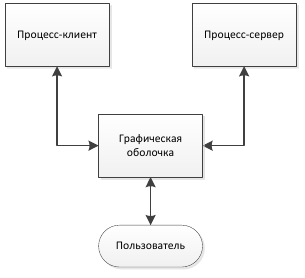
\includegraphics{pic_1}
    \caption{Структура программного обеспечения}\label{pic_1}
\end{figure}

На рисунке выше видно, что пользователь может взаимодействовать только с
графической оболочкой, графическая оболочка в свою очередь
взаимодействует с сервером и клиентом.

\subsection{Алгоритм работы клиента}
Приведем описание работы клиента. Описываемый здесь алгоритм клиента
не показывает взаимодействие клиента с остальными компонентами сети,
взаимодействие показано ниже. Приведем словесное описание того как
функционирует процесс, затем приведем схему алгоритма.
\newpar
Клиент запускается в момент запуска приложения, является процессом-демоном.
Процесс-клиент (или просто клиент) выполняет следующие
функции:
\begin{enumerate}
    \item при появлении в сети нового участника, клиент заносит его в список
        пассивных подключений;\label{enum:client}
    \item вызывает диспетчера (во время получения файла);\label{enum:disp}
    \item обрабатывает запросы, которые могли прийти от сервера или от
        GUI.\label{enum:gui}
\end{enumerate}

Ниже подробнее опишем данные функции.
\newpar
Рассмотрим последовательность действий выполняемых, когда клиент
получает сообщение от сервера или GUI (пункт \ref{enum:gui}). При получении
сообщения от GUI клиент вызывает обработчик запросов GUI и выполняет
некоторые действия, в числе которых может быть и завершение работы
клиента. Сообщение, получаемое клиентом от сервера, содержит кусок файла
и информацию, которая описывает каким образом обрабатывать данный
кусок файла. Данное сообщение передается callback-функции, которая
десериализует полученное сообщение и проверяет его на наличие ошибок,
если они присутствуют, то возвращается ошибка. Иначе происходит
идентификация пакета (определяется, какой уникальной передачи относится
получаемый пакет), если, идентификация неуспешна, то возвращается
ошибка, иначе вызывается функция, которая обрабатывает полученный кусок
файла. Данная функция выполняет следующие действия:
\begin{enumerate}
    \item если идентификатор файла отрицательное число, то возвращает
        управление и выводит сообщение об ошибке;
    \item иначе, копирует содержимое файла в список полученных кусков;
    \item если число подряд идущих кусков (то есть идентификаторы кусков
        расположены в списке в порядке возрастания) достигает
        определенной величины, то данные сбрасываются на жесткий диск.
\end{enumerate}

При получении некоторого куска файла он не сбрасывается на диск сразу, так
как в данном случае происходило бы частое обращение к жесткому диску
(запись данных на жесткий диск занимает относительно много времени, так
как связана с механическими действиями), что сказалось бы на общей
производительности.
\begin{figure}[!hbt]
    \centering
    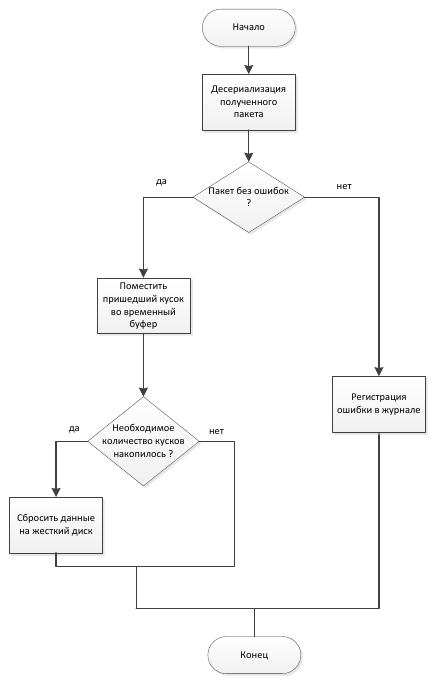
\includegraphics{pic_2_2}
    \caption{Блок-схема алгоритма процедуры обработки получаемых пакетов}\label{pic_2}
\end{figure}
\newpar
Для решения данной проблемы куски заносятся во
временный буфер, когда в буфере накапливается определенная
последовательность кусков, которые следуют друг за другом, то содержимое
сбрасывается на жесткий диск. На рисунке \ref{pic_2}, приведена блок-схема (далее
схема) алгоритма работы процедуры <<Обработчик данных>>, которая
обрабатывает получаемые пакеты.
\newpar
Другой функций клиента является добавление новых участников (пункт \ref{enum:client}).
\newpar
Если в сети появился новый участник, то вызывается функция, которая
добавляет этого участника в список пассивных подключений. Ниже, на
рисунке \ref{pic_3}, видно в какой момент происходит добавление нового участника
сети.

\begin{figure}[!hbtp]
    \centering
    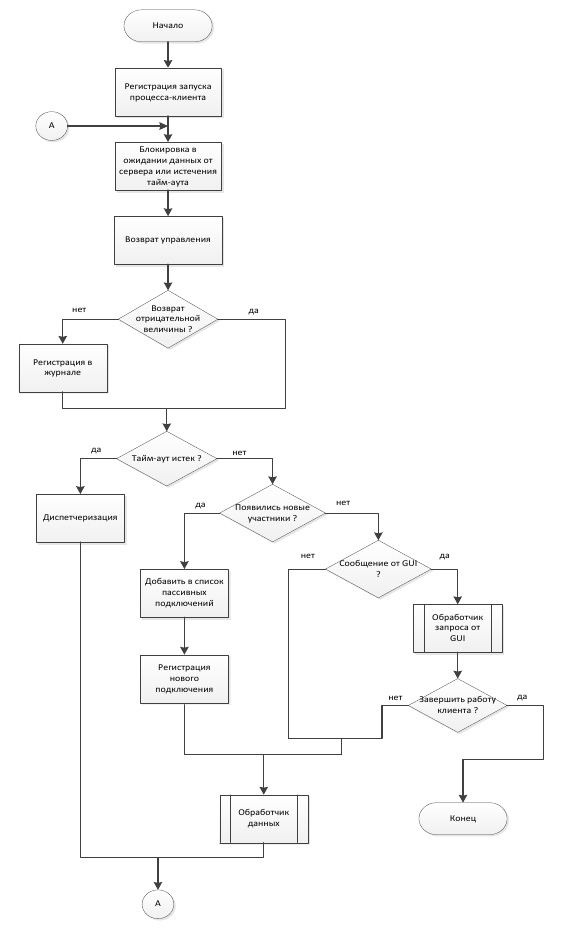
\includegraphics[scale=0.9]{pic_3}
    \caption{Блок-схема алгоритма работы клиента}\label{pic_3}
\end{figure}

\newpage
\subsection{Алгоритм работы сервера}
Приведем описание алгоритма работы сервера, который включает рассылку
широковещательных сообщений и передачу файлов при запросе от клиента.
Как и выше опишем алгоритм работы сервера словесно, а далее приведем
схему.
\newpar
Сервер, который, как и клиент является процессом-демоном, запускается в
момент запуска приложения. При этом процесс-сервер при запуске запускает
поток, тем самым работа сервера разделяется на следующие две задачи,
которые выполняются независимо друг от друга:
\begin{enumerate}
    \item поток, порожденный основным процессом, производит рассылку
        широковещательных сообщений всем участникам сети;
    \item основной процесс ожидает получения запроса на передачу
        некоторого куска.
\end{enumerate}

Поток, отвечающий за рассылку широковещательных сообщений,
порождается сразу при запуске основного процесса-сервера. После удачного
запуска он производит широковещательную рассылку сообщений участникам
сети.
\newpar
Основной процесс после удачного запуска ожидает запроса на передачу
некоторого файла, который посылается некоторым участником сети.
Ожидание происходит путем блокирования процесса на системном вызове
select. Данный системный вызов используется для организации
мультиплексирования ввода-вывода, который описывается далее. Когда
сервер получает сообщение от клиента, которое также является
последовательностью байтов и содержит информацию о куске файла который
необходимо передать клиенту, он (сервер) проверяет наличие файла на хосте.
В случае успеха он считывает кусок файла и передает его клиенту, иначе
передает клиенту сообщение об ошибке, то есть информирует клиента о том,
что запрашиваемый файл отсутствует.
\newpar
Ниже, на рисунке \ref{pic_4} приведем общую схему работы основного процесса-сервера,
схема работы потока приводиться не будет, так как алгоритм
достаточно простой. Также как и в процессе-клиенте, используется системная
функция select, которая может вернуть отрицательное значение. Данный факт
будет регистрироваться в журнале, однако процесс-сервер не будет прерывать
свою работу, так как данная ошибка не является критической.

\begin{figure}[!p]
    \centering
    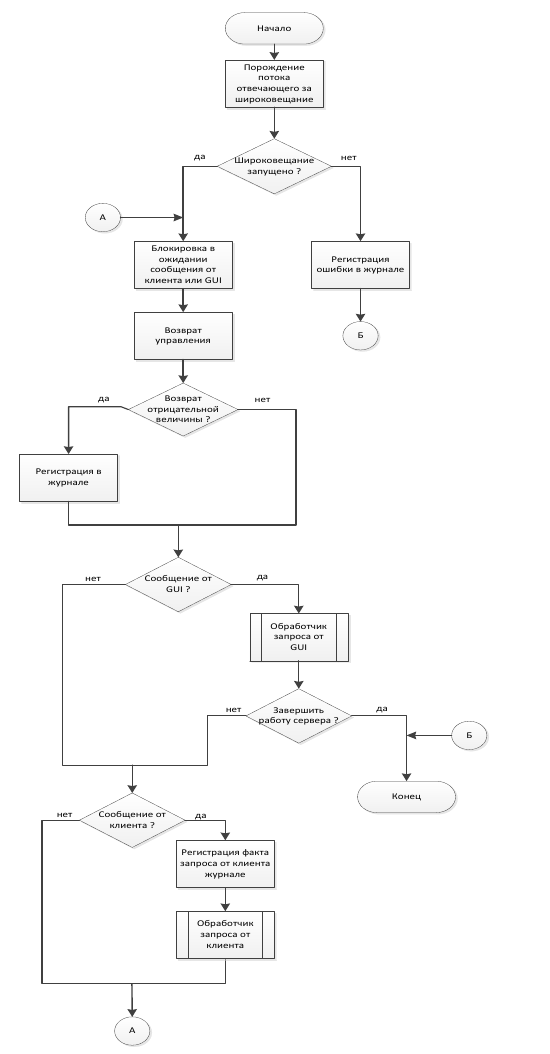
\includegraphics[scale=0.88]{pic_4}
    \caption{Блок-схема алгоритма работы сервера}\label{pic_4}
\end{figure}

\newpar
Процедура, которая обрабатывает запросы пришедшие серверу, будет описана
ниже на рисунке \ref{pic_5}, также будет приведена схема этой процедуры.

\begin{figure}[!p]
    \centering
    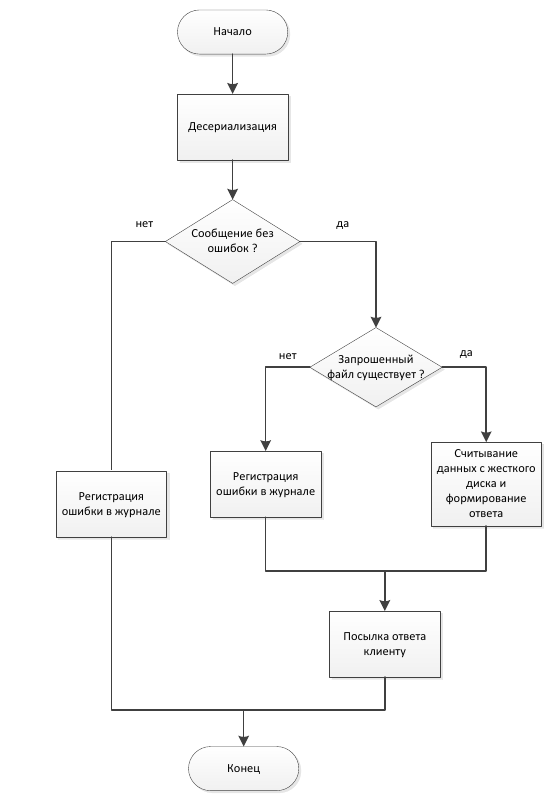
\includegraphics[width=\textwidth]{pic_5}
    \caption{Блок-схема алгоритма процедуры обработки запроса сервером}\label{pic_5}
\end{figure}

\newpar
На схеме, приведенной на рисунке \ref{pic_4}, происходит вызов процедуры <<Обработчик
запроса от клиента>>, данная процедура обрабатывает запросы, пришедшие от
других участников сети. Опишем алгоритм работы данной процедуры.
\newpar
Процедура <<Обработчик запроса от GUI>> принимает и обрабатывает
сообщение от GUI, которое может быть только сообщением о завершении
работы сервера.
\newpar
При вызове процедуры обработки запроса от клиента ей передается
сообщение, а именно протокол в виде последовательности байт. Далее
происходит десериализация, если она успешна, то процедура продолжает
работу, иначе выход с ошибкой. Ошибка может произойти, если полученное
сообщение имеет неверный формат, иначе происходит обработка запроса и
формирование ответа. При формировании ответа сервер проверяет наличие
запрашиваемого файла и в случае успеха пересылает клиенту тот кусок
файла, который запросил клиент, иначе передается сообщение об ошибке.
\newpar
На рисунке \ref{pic_5}, приведена схема работы процедуры обработки запроса.

\subsection{Взаимодействие с пользовательским приложением}
В основном, взаимодействие сервера и клиента с графической оболочкой
сводится к обмену некоторой информацией о состоянии передачи или число
участников в сети.
\newpar
Перед началом передачи файла клиент должен получить информацию о том
файле, который необходимо запросить у серверов. Данная информация
передается клиенту пользовательским приложением
(графической оболочкой). Для этого использовался текстовый формат передачи данных
JSON.

\subsection{Взаимодействие клиента и сервера}
Выше были описаны алгоритмы работы клиента и сервера, а также
получение запроса на передачу файла. Теперь опишем алгоритм
взаимодействия клиента и сервера. Подразумевается, что клиент и сервер
находятся на разных хостах.
\newpar
Когда необходимо получить некоторый файл клиент получает информацию о
нем из пользовательского приложения (GUI). Получив информацию о файле,
который необходимо получить, клиент заносит всех из списка пассивных
подключений в список активных подключений, далее проходит по списку
активных подключений, и посылает каждому запрос на передачу куска файла,
который необходимо получить. Сервер, получив запрос от клиента на
передачу куска файла, проверяет наличие файла на хосте и в случае успеха
пересылает клиенту запрашиваемый кусок файла. Иначе посылает
сообщение, в котором указано, что на данном сервере нет запрашиваемого
файла. Клиент начинает получать различные куски файлов и действует
согласно выше описанному алгоритму. Если какой-либо сервер присылает
сообщение об отсутствие файла, клиент удаляет из списка активных
соединений, то есть в последствие не запрашивает данный файл у этого
сервера. Во время передачи файла может возникнуть ситуация, когда
некоторый сервер не отвечает определенное время либо завершил свою
работу, не переслав необходимые данные. В таком случае, кусок файла
возвращается в список запрашиваемых кусков и будет запрошен повторно.

\subsection{Алгоритм планирования}
Опишем алгоритм планирования запросов для получения кусков.
\newpar
Данный алгоритм реализуется клиентом. Размер куска файла определяется
как некоторая константа. Планирование происходит по следующим правилам:
\begin{enumerate}
    \item клиент логически разбивает файл на куски, каждый из которых
        имеет одинаковый размер;
    \item каждый кусок нумеруется в порядке возрастания;
    \item следующим будет запрошен минимальный кусок из списка
        отвергнутых кусков, если он не пуст, иначе кусок с минимальным
        порядковым номером, который еще не был запрошен;
    \item если некоторый кусок, не может быть получен от сервера, то он
        помещается в список отвергнутых кусков для того, чтобы быть
        запрошенным как можно раньше.
\end{enumerate}

\subsection{Алгоритм функционирования приложения}
Ниже, на рисунках \ref{pic_6}, \ref{pic_7} и \ref{pic_8} приведем блок-схему функционирования приложения,
при этом в ней не будем приводить алгоритмы функционирования клиента и
сервера, так как они приведены выше. То есть, данная схема отображает
только логику работы приложения.

\begin{figure}[!p]
    \centering
    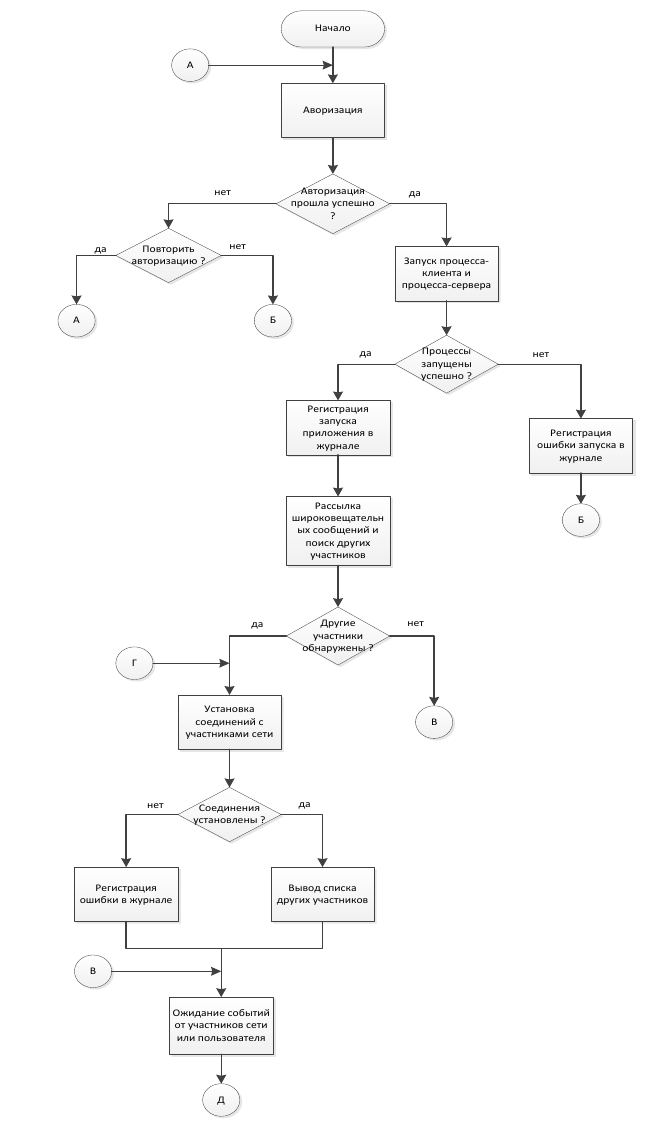
\includegraphics[scale=0.8]{pic_6}
    \caption{Блок-схема алгоритма функционирования приложения}\label{pic_6}
\end{figure}

\begin{figure}[!p]
    \centering
    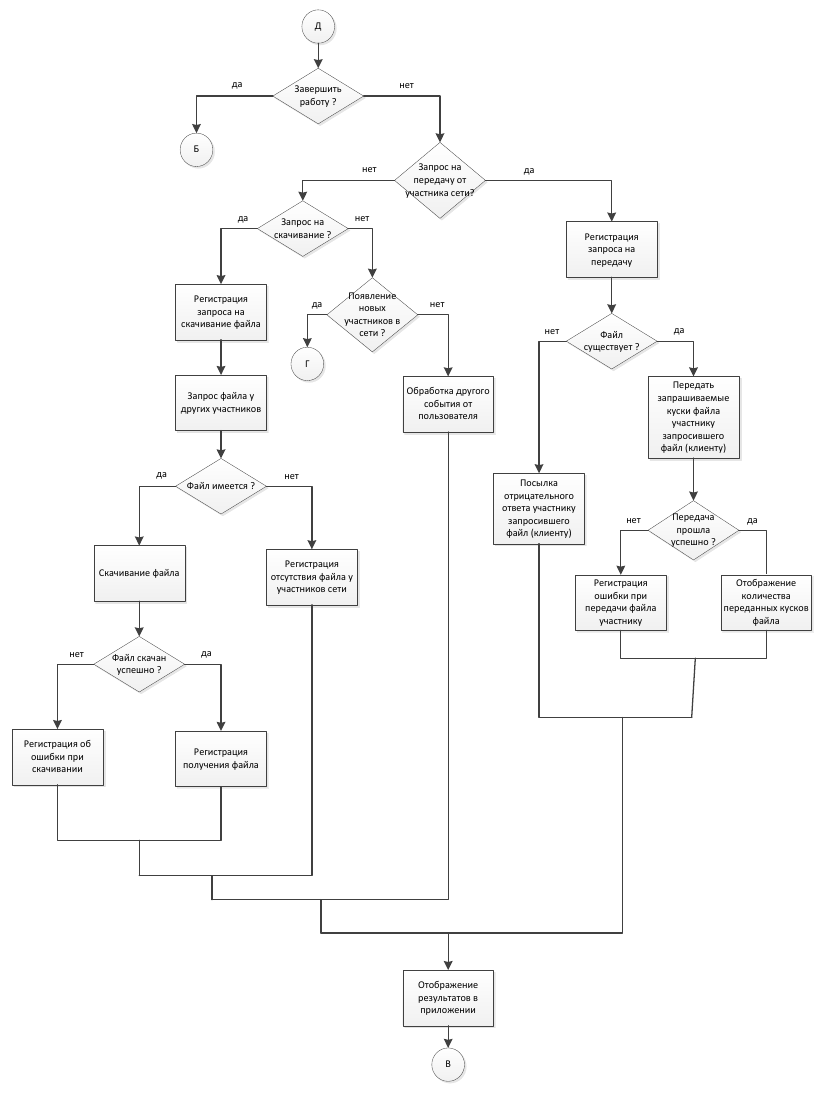
\includegraphics[scale=0.8]{pic_7}
    \caption{Блок-схема алгоритма функционирования приложения (продолжение)}\label{pic_7}
\end{figure}

\newpage
\begin{figure}[t!]
    \centering
    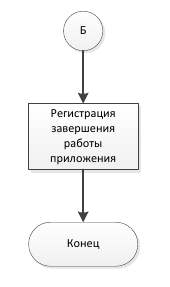
\includegraphics[scale=0.8]{pic_8}
    \caption{Блок-схема алгоритма функционирования приложения (продолжение)}\label{pic_8}
\end{figure}

\subsection{Схема взаимодействия участников сети}
Приведем схему взаимодействия в сети, на которой отобразим то, как
происходит взаимодействие между участниками сети.
\newpar
Под участником сети здесь будем понимать приложение, которое было
запущено на хосте. Как описывалось выше, каждое приложение состоит из
процесса-клиента, процесса-сервера и пользовательского приложения,
которое предоставляет графический интерфейс пользователю.
\newpar
Ниже, на рисунке \ref{pic_9}, приведена схема взаимодействия нескольких участников сети. На
этой схеме, процесс-сервер и процесс-клиент показаны в блоках <<Сервер i>> и
<<Клиент i>> соответственно. Блок пользовательского приложения имеет
соответствующее название <<Пользовательское приложение i>>, где i~-- номер
участника сети. Стрелками будем указывать направления обмена
сообщениями. Номера стрелок соответствуют следующим сообщениям:
\begin{enumerate}
    \item посылка широковещательного сообщения всем участникам сети,
        широковещание производится сервером, передача куска файла запрошенного
        клиентом или посылка сообщения о том, что у данного сервера отсутствует
        запрашиваемый файл.
    \item сообщения от других участников сети. Сообщение может информировать
        о появлении в сети нового участника, то есть перехват широковещательного
        сообщения посланного сервером, передаваемый кусок файла, который был
        предварительно запрошен у сервера (стрелка 1), а также сообщение об
        отсутствие запрашиваемого файла.
    \item обмен сообщениями между сервером и пользовательским приложением,
        со стороны сервера приходит информация о текущих передачах, например
        число передаваемых кусков файла или скорость передачи и т.д. Со стороны
        пользовательского приложения приходит сигнал о завершении работы.
    \item обмен сообщениями между пользовательским приложением и клиентом.
        Со стороны клиента присылается информация о текущей передаче, например
        скорость передачи, число принятых пакетов, адреса участников, чьи
        широковещательные сообщения были перехвачены и т.д. Со стороны
        приложения клиенту посылается сигнал о завершении работы или
        информация о том файле, который необходимо запросить у других
        участников.
\end{enumerate}

\begin{figure}[tb!]
    \centering
    \hspace*{-2cm}
    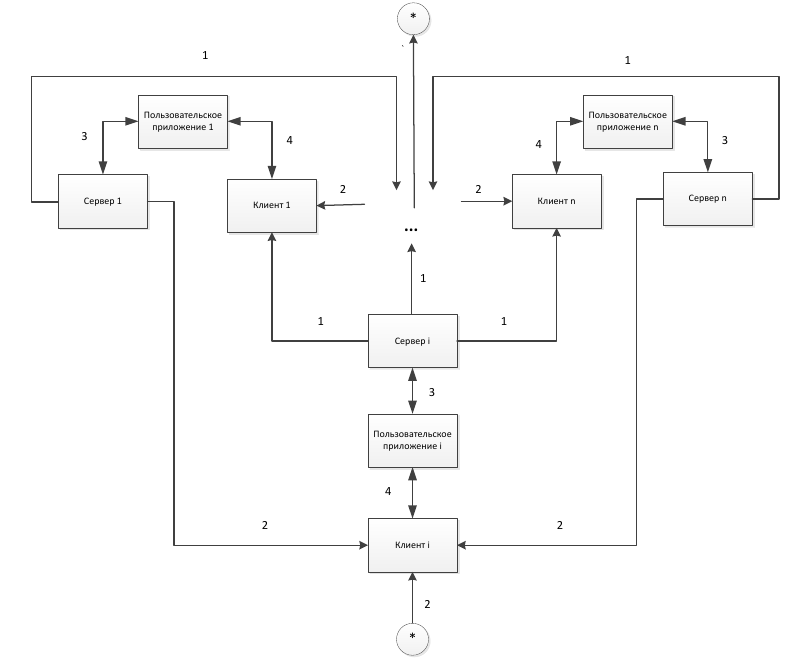
\includegraphics[scale=0.9]{pic_9}
    \caption{Схема взаимодействия между участниками сети}\label{pic_9}
\end{figure}

На рисунке \ref{pic_10}, ниже представим схему взаимодействия некоторого i-го
участника сети с другими участниками сети и покажем обмен сообщениями
между ними. Пунктирной линией по центру выделен некоторый i-й участник.
Видно как происходит запрос на передачу файла у других участников сети, а
именно у серверов, которые указаны справа. Слева и справа от i-го участника
также располагаются такие же участники, однако они показаны частично,
например, справа можно видеть лишь серверные составляющие остальных
участников сети. Также показан обмен сообщениями между клиентом и
сервером с пользовательским приложением, которое обозначено как GUI.

\begin{figure}[tb!]
    \centering
    \hspace*{-2cm}
    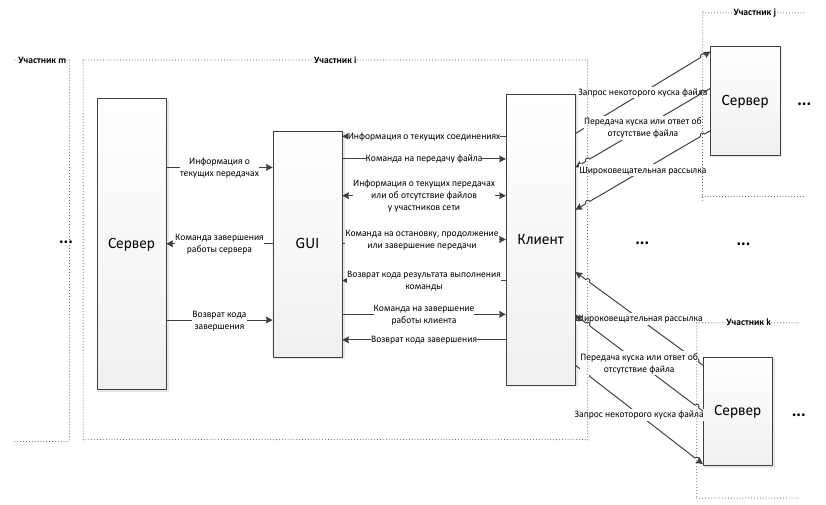
\includegraphics[scale=0.9]{pic_10}
    \caption{Схема взаимодействия между участниками и компонентами приложения}\label{pic_10}
\end{figure}

\subsection{Протокол}
Протокол разрабатывался с учетом описанных выше алгоритмов работы
клиента и сервера. Протокол представлен в виде структуры. Ниже
представим и опишем назначения полей структуры.
\begin{figure}
    \begin{lstlisting}[language=C]
struct cli_fields {
    pack_id_t pack_id;
    piece_id_t piece_id;
    perror_t error;
    file_id_t file_id;
    unsigned char hsumm[MD5_DIGEST_LENGTH];
    char file_name[FILE_NAME_MAX_LEN];
};
    \end{lstlisting}
\end{figure}
\newpar
Структура cli\_fields используется при передаче сообщения от клиента
серверу. Первое поле структуры pack\_id содержит значение номера
передаваемого пакета. Поле piece\_id равно номеру передаваемого куска. Поле
error содержит некоторое значение ошибки. Поле file\_id содержит
идентификатор файла и при передаче серверу клиентом всегда равно -1, по
данному идентификатору и номеру передаваемого куска можно однозначно
идентифицировать передачу. Далее следует поле hsumm, которое содержит
хэш-сумму передаваемого файла, оно (поле) составляет 16 байт и
генерируется стандартным алгоритмом md5. Последнее поле file\_name
содержит имя запрашиваемого файла. Необходимо заметить, что в данной
структуре отсутствует поле для данных, так как в нем нет необходимости.
Клиенту не нужно передавать данные серверу, так как он запрашивает файл.
\begin{figure}[h!]
    \begin{lstlisting}[language=C]
struct srv_fields {
    struct cli_fields cli_field;
    size_t piece_len;
    unsigned char piece[DATA_BLOCK_LEN];
};
    \end{lstlisting}
\end{figure}
\newpar
Следующая структура передается от сервера клиенту. Первое поле cli\_field
является структурой, которую клиент передает серверу, данные в этой
структуре такие же за исключением того, что поле file\_id равно некоторому
целому значению. Следующее поле piece\_len равно длине передаваемого
куска клиенту сервером. Поле piece содержит в себе кусок файла, то есть
передаваемые данные.

\subsection{Использование протокола для обмена сообщениями}
\begin{figure}[tb!]
    \centering
    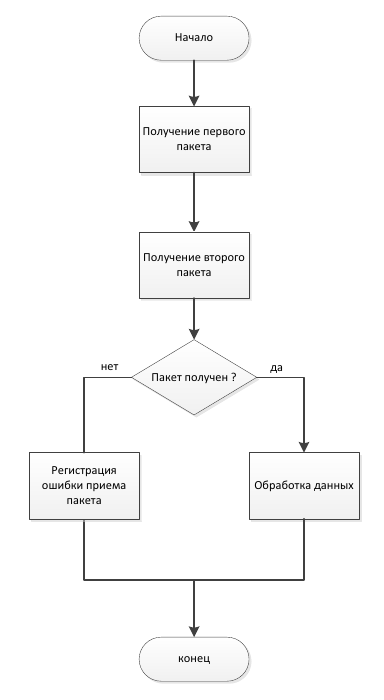
\includegraphics[scale=0.8]{pic_11}
    \caption{Блок-схема алгоритма получения пакетов}\label{pic_11}
\end{figure}
В процессе своей работы клиент и сервер обмениваются сообщениями,
которые содержат данные и информацию о том, как эти данные обрабатывать.
Протокол представлен в виде структуры, поэтому перед передачей структуру
необходимо преобразовать в последовательность байт, то есть сериализовать,
и десериализовать при получении, то есть преобразовать полученную
последовательность байтов в структуру. Однако так как размер передаваемой
последовательности (или сообщения) может быть различным (так как может
передаваться кусок файла), то необходимо преждевременно уведомить
принимающую сторону о размере передаваемого пакета (последовательности
байт). Для реализации этого передаются два пакета, первый пакет имеет
определенный размер и содержит в себе длину второго пакета. При такой
организации, принимающая сторона предварительно получает данные о
размере второго (основного) пакета. Заметим, что передачу можно
реализовать при помощи посылки одного пакета и дожидаться, когда будет
получен тот объем данных, который содержит размер всего пакета, и на
основе полученной информации продолжить ожидать получение основного
пакета, однако, был выбран первый способ, основанный на передачи двух
пакетов.
\newpar
На рисунке \ref{pic_11}, приведена схема алгоритма получения пакета.
\subsection{Мультиплексирование ввода-вывода}
Мультиплексирование ввода-вывода необходимо для того, чтобы
обрабатывать запросы, которые приходят от клиентов или серверов
участников сети. Данный механизм реализован при помощи системного
вызова select. Смысл мультиплексирования заключается в том, что процесс-
клиент или процесс-сервер блокируются на системном вызове до тех пор,
пока кто-нибудь из участников сети не пошлет некоторый запрос. После того,
как процесс-сервер или процесс-клиент получили хотя бы один запрос,
системный вызов select, на котором был заблокирован процесс-сервер или
процесс-клиент, возвращает управление. После чего анализируется
множество и делается вывод, от какого из участников пришел запрос, далее
данный запрос обрабатывается соответствующим образом. Данный механизм
ввода-вывода позволяет сэкономить на том, что нет необходимости постоянно
опрашивать всех участников на наличие пришедших запросов от них, а также
позволяет обработать случай, когда одновременно пришли два или более
запросов.
\subsection*{Выводы}
\addcontentsline{toc}{subsection}{Выводы}
Программное средство состоит из клиентской и серверной частей, а также из
пользовательского приложения. Пользовательское приложение предназначено
для предоставления доступа к основным функциям программного
обеспечения и взаимодействует с клиентской и серверной частями, которые
обеспечивают функции клиента и сервера соответственно. Под функциями
клиента понимается запрос на предоставление некоторого файла и
последующее скачивание. Под функциями сервера понимается передача
запрошенного файла, если он имеется на данном хосте. Программное
обеспечение разработано в соответствие со структурной методологией.

	\section{Технологическая часть}
\newsection{Технологическая часть}

\subsection{Выбор языка программирования и среды разработки}
В качестве среды программирования была выбрана операционная система
GNU/Linux. Данная операционная система распространяется по лицензии
GNU GPL и поддерживает стандарт POSIX, поэтому, программное
обеспечение, разрабатываемое для данной операционной системы, будет
переносимо на другие платформы, которые поддерживают POSIX. Также,
одним из преимуществ данной операционной системы является открытость
исходных кодов, что в некоторых случаях позволит более подробно изучить
особенности используемых системных функций. Отлаживать программное
обеспечение в GNU/Linux намного проще, так как нет проблем связанных
политикой безопасности различных антивирусных программ, что присуще
операционной системе Windows.
\newpar
Для реализации программного обеспечения использовался язык C. Данный
язык обладает удобством высокоуровневых языков и возможностями
низкоуровневых языков, что при правильном использовании даст хороший
результат с точки зрения производительности и использования памяти, что в
свою очередь сделает программное обеспечение менее требовательным к
ресурсам и повысит переносимость. Недостатком данного языка является
сложность отладки кода, однако существует различные отладчики, что
упрощает данную проблему.
\newpar
Для создания пользовательского приложения использовался язык Python, версии 3.3,
который более удобен для разработки пользовательского
интерфейса.
\newpar
В число используемых средств также вошли: текстовый редактор vim для
редактирования исходных кодов программы, утилита make для компиляции
исходных кодов и последующей компоновки, отладчик gdb для отладки
программного обеспечения.
\subsection{Описание модулей программного обеспечения}
В данном разделе опишем основные назначения модулей программного
обеспечения. Прототипы и описание пользовательских функций и структур
будут приведены в разделе <<Приложение А>>. Отметим, что алгоритмы работы
этих пользовательских функций описаны в конструкторской части, здесь
же приведена их технологическая составляющая. Используемые типы и
константы приведем в данном разделе. В раздел <<Приложение А>> также
вынесены константы, которые определены в дополнительных файлах.

\subsubsection*{Модуль Network}
Исходные коды данного модуля представлены в файле \textit{network.c}, прототипы
приведены в файле \textit{network.h}. Назначением данного модуля является
установление связи с участниками сети, периодическая посылка
широковещательных сообщения, перехват событий связанных с отправкой и
приемом сообщений. Данный модуль также производит вызов callback-функций
при получении сообщения от сервера или клиента.
\newpar
В данном модуле определены два типа, которые являются указателями на
callback-функции. Данные указатели содержат адреса обработчиков, которые
вызываются, когда необходимо обработать сообщение, пришедшее от клиента
или сервера. Обе функции возвращают целочисленные значения, если оно
равно нулю, то ошибок нет, иначе в зависимости от ненулевого значения
выдается соответствующая ошибка. Ниже приведем определение данных
типов.
\begin{lstlisting}[language=C]
typedef int (*socket_callback)(int sender_sock, const char *received_data, size_t data_len);
typedef int (*server_response_callback)(struct sockets_queue *queue);
\end{lstlisting}
\newpar
Также здесь определены константы, число одновременно прослушиваемых
сокетов, максимальное количество устанавливаемых соединений, и строка
для аутентификации, соответственно.
\begin{lstlisting}
#define SELECT_QUEUE_LEN        5
#define MAX_INTERFACES_COUNT    16
#define IDENT_MSG     "Dzhumagulov_Berezhnoy_IU_7_2013"
\end{lstlisting}

\subsubsection*{Модуль Proto}
Исходный код данного модуля представлен в файле \textit{proto.c}, а прототипы
используемых функций описаны в файле \textit{proto.h}. В данном модуле
описываются правила интерпретации передаваемых сообщений, то есть
протокол, и функции для обработки этих сообщений, а именно функции,
которые преобразуют данные из структуры в последовательность байт или из
последовательности байт получают данные, которыми заполняется структура.
Также имеется дополнительная функция для проверки отдельных бит на
наличие ошибок.
\newpar
Опишем следующие типы:
\begin{lstlisting}
typedef unsigned int pack_id_t; \\ Идентификатор пакета
typedef unsigned int piece_id_t;\\ Идентификатор куска файла
typedef signed int file_id_t;   \\ Идентификатор файла
typedef unsigned short perror_t;\\ Байт для идентификации ошибок
typedef unsigned long long piece_len_t;\\ Длина пересылаемого куска файла
\end{lstlisting}

Соответственно выше определенным типам сопоставляются константы.
\begin{lstlisting}
#define PACK_ID_TSIZE sizeof(pack_id_t)
#define PIECE_NUM_TSIZE sizeof(piece_id_t)
#define FILE_NUM_TSIZE sizeof(file_id_t)
#define PIECE_LEN_TSIZE sizeof(piece_len_t)
#define PROTOCOL_ERROR_TSIZE sizeof(perror_t)
\end{lstlisting}

Ниже представлены номера битов для интерпретации определенных ошибок
протокола.
\begin{lstlisting}
#define PE_FOPEN_FAILURE        0   \\ Ошибка открытия файла
#define PE_FILE_NOT_EXISTS      1   \\ Файл отсутствует на хосте
#define PE_HASH_CMP_FAILURE     2   \\ Неверная хэш-сумма
#define PE_TRNMS_CMPL           3   \\ Передача завершена
#define PE_READ_ACCESS_DENIED   4   \\ Ошибка при попытке прочитать файл
\end{lstlisting}

\subsubsection*{Модуль Cli}
Исходный код и прототипы приведены в \textit{cli.c} и \textit{cli.h} соответственно. В
данном модуле реализован алгоритм работы клиента, а именно алгоритм
реализующий распределение запросов для получения кусков файла, и их
дальнейшую обработку. Ниже приведем используемые константы.
\begin{lstlisting}
#define SRV_UNKN                0   \\ Сервер недоступен
#define SRV_READY               1   \\ Сервер готов к передаче
#define SRV_BUSY                2   \\ Сервер занят


#define TRM_WAITING_SERVERS     0   \\ Ожидание серверов
#define TRM_OBTAINING           1   \\ Получение файла
#define TRM_COMPLETED           2   \\ Передача завершена
#define TRM_UNKN                3   \\ Ошибка при передаче


#define TRME_TOO_MANY_TRM      -1   \\ Слишком много передач
#define TRME_DECODE_ERR        -2   \\ Ошибка при создании сообщения
#define TRME_SOCKET_FAILURE    -3   \\ Возникла ошибка на сокете
#define TRME_NO_ACTIVE_SRVS    -4   \\ Ни один сервер не смог получить запрос
                                    \\ на передачу
#define TRME_ALLOC_FAILURE     -5   \\ Ошибка при выделении памяти
#define TRME_FILE_ERROR        -6   \\ Ошибка при работе с файлом
#define TRME_OUT_OF_MEMORY     -7   \\ Не хватает памяти для всего файла
#define TRME_OPTS_FAILURE      -8   \\ Ошибка при передаче аргуметов
\end{lstlisting}

\subsubsection*{Модуль Srv}
Исходный код приведен в \textit{src.c}, прототипы приведены в \textit{srv.h}. В данном
модуле реализован алгоритм работы сервера. Сервер производит
широковещание через определенный промежуток времен, а при наличии
запрашиваемого файла и соответствующего запроса от клиента начинает
передачу куска файла клиенту. Прототипы функций и структуры приведены
в приложении А.

\subsubsection*{Модуль JSON и MD5}
Данные модули предоставляют стандартные функции для получения хеш-сумм
(модуль MD5) и функций для обмена данными JSON.

\subsubsection*{Модуль Main}
Данный модуль используется для запуска процессов сервера и клиента.
Также содержит функцию, которая позволяет перевести процесс в фоновый
режим работы.

\subsection{Потенциальные ошибки}
В результате работы приложения могут происходить те или иные ошибки,
которые необходимо обрабатывать. Далее рассмотрим основные ошибки и
их обработку.
\begin{enumerate}
    \item Ошибки, возникающие при работе с системными функциями. Данные
        ошибки возникают в результате вызова используемых системных
        функций, например открытие файла, чтение файла или запись в файл, а
        также функция используемые для мультиплексирования ввода\\вывода,
        системные функции, используемые для работы с сокетами и так далее.
        \newpar
        Причиной некорректной работы могут быть, хотя и маловероятно,
        ошибки, возникающие в ходе работы операционной системы,
        неполадки с сетью, или неверные параметры, передаваемые этим
        функциям. В данном случае, если ошибки возникли в результате
        неполадок с ОС, то поведение приложения непредсказуемо, ошибки
        возникающие в результате передачи неверных параметров,
        обрабатываются таким образом, чтобы не нарушалась работа
        приложения, но, если ошибка критическая, то работа приложения
        завершается и выдается сообщение об ошибке. Если ошибки возникают
        из-за неполадок в сети, то работа приложения также завершается.
        \newpar
        Сюда же можно включить ошибки связанные с неполадками в аппаратуре,
        данные ошибки невозможно предусмотреть, поэтому они не
        обрабатываются.
    \item Ошибки, возникающие при завершении работы участников сети.
        Данные ошибки возникают из-за того, что в любой момент времени
        любой из участников сети может завершить работу, в момент передачи
        или приема некоторого файла. Результат обработки таких ошибок
        зависит от количества участников, которые обмениваются файлами.
        \newpar
        Так, если клиент, принимающий файл завершил свою работу, то
        завершают работу все серверы, которые передавали файл этому
        клиенту, если при завершении работы сервера, остаются другие
        работающие сервера, то передача не завершается и не выдается
        сообщение об ошибке, однако когда количество таких серверов равно
        нулю, то клиент завершает работу с ошибкой. В таком случае
        пользовательское приложение выводит сообщение об ошибке.
    \item  Ошибки, возникающие в результате некорректного завершения
        пользовательских функций. Данные ошибки происходят в ситуациях,
        когда пользовательская функция не в состоянии корректно завершить
        свою работу из-за невозможности правильной интерпретации входных
        данных.
        \newpar
        Такие ошибки могут возникать в результате сериализации и
        десериализации сообщений, которыми обмениваются участники, при
        повторном запуске приложения на одном и том же хосте, при
        превышении некоторых ограничений, например при попытке, запустить
        большее количество передач, чем это возможно. При возникновении
        таких ошибок, пользовательские функции возвращают код ошибки,
        которая интерпретируется особым образом. В результате приложение
        выдает сообщение об ошибке или продолжает работу, если ошибка не
        влияет на работу приложения. Например, попытка повторного запуска
        приложения, не влияет на ход работы первого, уже запущенного
        приложения.
\end{enumerate}

\setcounter{figure}{0}
\subsection{Описание графического интерфейса}
Здесь опишем графический интерфейс.
\newpar
При старте пользовательского приложения необходимо ввести логин и
пароль, как это показано ниже на рисунке \ref{login_window}.
\begin{figure}[!hbt]
    \centering
    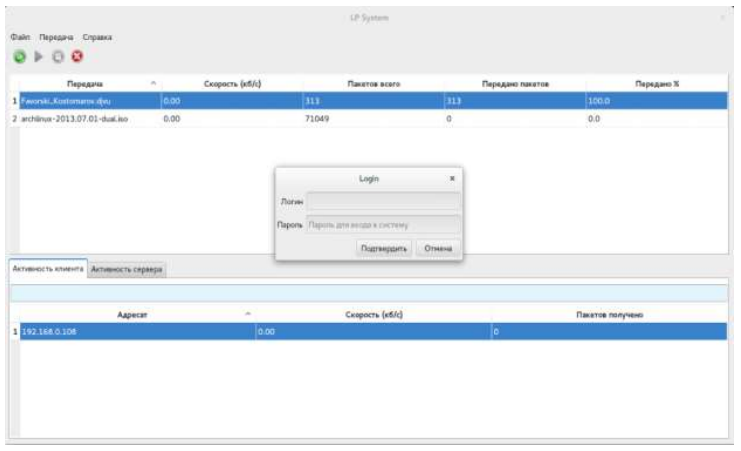
\includegraphics[width=\textwidth]{login}
    \caption{Авторизация}\label{login_window}
\end{figure}
\newpar
В случае ошибки авторизации выводится сообщение, изображенное на рисунке \ref{auth_err}.
\begin{figure}[!hbt]
    \centering
    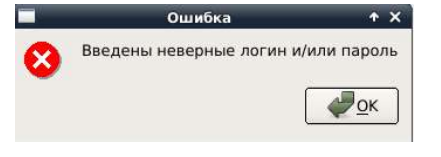
\includegraphics{auth_err}
    \caption{Сообщение об ошибке авторизации}\label{auth_err}
\end{figure}
\newpar
После успешной авторизации, становится доступным главное окно. В
главном окне, имеются следующие основные компоненты:
\begin{enumerate}
    \item главное меню --- содержит три вкладки;
    \item окно передач --- окно содержит информацию о текущих передачах;
    \item окно для просмотра активностей с вкладками <<Активность клиента>> и <<Активность сервера>>;
    \item дополнительная панель с кнопками управлениями.
\end{enumerate}

Главное меню приведено на рисунке \ref{main_menu}. При нажатии на вкладки появляются
выпадающее меню. Выпадающее меню <<Файл>> содержит лишь кнопку для
выхода (рисунок \ref{exit_btn}).

\begin{figure}[!hbt]
    \centering
    
\includegraphics{main_menu}
    \caption{Главное меню приложения}\label{main_menu}
\end{figure}
\begin{figure}[!hbt]
    \centering
    
\includegraphics{exit_btn}
    \caption{Выпадающее меню <<Файл>>}\label{exit_btn}
\end{figure}

При нажатии на вкладку <<Передача>>, появляется выпадающее меню, которое
показано на рисунке \ref{transmit}. Для добавления нового торрент файла необходимо
выбрать пункт <<Создать торрент файл>>, при этом появляется окно, куда
необходимо внести информацию о файле, окно представлено на рисунке \ref{add_torrent}.

\begin{figure}[!hbt]
    \centering
    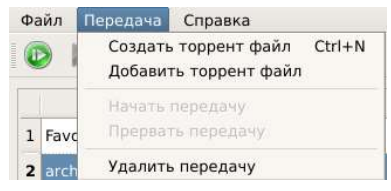
\includegraphics{transmit}
    \caption{Выпадающее меню <<Передача>>}\label{transmit}
\end{figure}
\begin{figure}[!hbt]
    \centering
    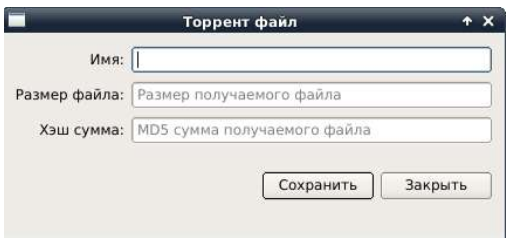
\includegraphics{add_torrent}
    \caption{Диалог создания нового торрент файла}\label{add_torrent}
\end{figure}

Для добавления торрент файла, который уже существует, необходимо выбрать
соответствующий пункт меню <<Добавить торрент файл>>. При этом
появляется стандартное окно, в котором можно будет выбрать необходимый
файл. Пункт <<Удалить передачу>> удаляет передачу, выделенную в окне
передач. Пункты <<Начать передачу>> и <<Прервать передачу>> позволяют начать
и прервать передачу, соответственно.
\newpar
Ниже приведено выпадающее меню вкладки <<Справка>> (рисунок \ref{help}). Пункт
<<Разработчики>> выводит окно, в котором отображается информация о
разработчиках данного программного обеспечения (рисунок \ref{about}).
\begin{figure}[!hbt]
    \centering
    
\includegraphics{help}
    \caption{Выпадающее меню <<Справка>>}\label{help}
\end{figure}
\begin{figure}[!hbt]
    \centering
    
\includegraphics{about}
    \caption{Окно <<Разработчики>>}\label{about}
\end{figure}

При выборе пункта <<История>> появляется окно журнала, в котором
содержится информация об основных событиях системы, таких как
возникшие ошибки, сообщения о запуске приложения, обнаружение новых
участников и т.д. Пример приведен на рисунке \ref{hist}.

\begin{figure}[!hbt]
    \centering
    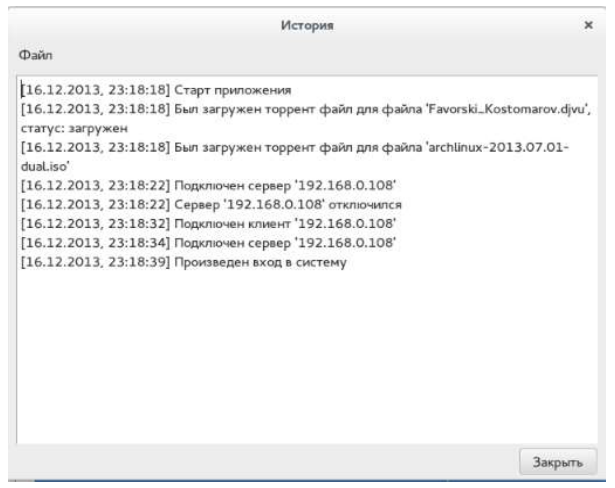
\includegraphics{hist}
    \caption{Окно <<История>>}\label{hist}
\end{figure}

Дополнительная панель с кнопками управления, приведенная на рисунке \ref{buttons},
добавлена для удобства и выполняет те же действия, что и описанные выше
пункты выпадающего меню <<Передача>>, поэтому не будем повторно
описывать их назначение.

\begin{figure}[!hbt]
    \centering
    
\includegraphics{buttons}
    \caption{Панель с кнопками управления}\label{buttons}
\end{figure}

Окно передач содержит сведения о передачах. В данном окне, рисунок \ref{transmitions},
отображается следующая информация:
\begin{enumerate}
    \item скорость передачи (кб/с) -- отображает скорость передачи;
    \item общее количество пакетов -- число пакетов, составляющих некоторую
        передачу;
    \item переданное количество пакетов -- число переданных пакетов на данный
        момент;
    \item процент переданного пакета (\%) -- какая часть передана.
\end{enumerate}

\begin{figure}[!hbt]
    \centering
    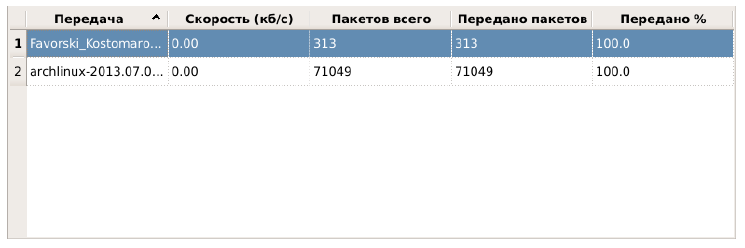
\includegraphics[width=\textwidth]{transmitions}
    \caption{Окно передач}\label{transmitions}
\end{figure}

На рисунке \ref{transmitions} видны две полностью завершенные передачи.
Окно для просмотра активностей с вкладками <<Активность клиента>> на
рисунке \ref{cli_act} и <<Активность сервера>> на рисунке \ref{srv_act} ниже.

\begin{figure}[!hbt]
    \centering
    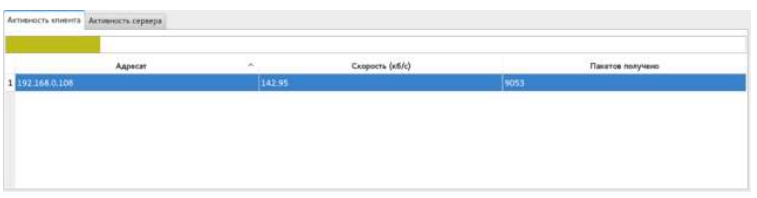
\includegraphics[width=\textwidth]{cli}
    \caption{Вкладка <<Активность клиента>>}\label{cli_act}
\end{figure}

Вкладка <<Активность клиента>> отображает информацию об активности, а
именно:
\begin{enumerate}
    \item адресат -- кто присылает данные;
    \item скорость (кб/с) -- скорость передачи;
    \item пакетов получено – число полученных пакетов.
\end{enumerate}

\begin{figure}[!hbt]
    \centering
    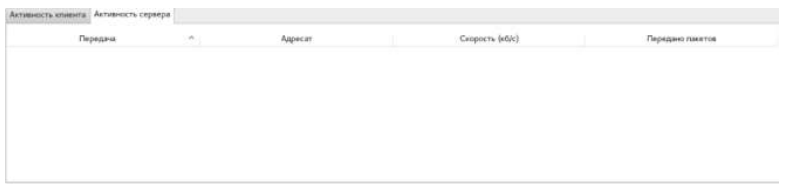
\includegraphics[width=\textwidth]{srv}
    \caption{Вкладка <<Активность сервера>>}\label{srv_act}
\end{figure}

Вкладка <<Активность сервера>>, отображает информацию о серверах,
которые передают файл, в данной вкладке отображается следующая
информация:
\begin{enumerate}
    \item передача -- к какой передаче относится сервер;
    \item адресат -- кому пересылается;
    \item скорость (кб/с) -- скорость передачи;
    \item передано пакетов -- число переданных пакетов.
\end{enumerate}

\subsection{Тестирование программного обеспечения}
Здесь приведем результаты
 тестирования программного обеспечения. В
 результате тестирования
  необходимо убедиться, что программное
  обеспечение удовлетворяет
   основным требованиям, а также адекватно
   реагирует на внештатные
    ситуации, которые могут возникнуть. Для
    тестирования были использованы три операционные системы Linux Debian,
    которые были запущены на виртуальных машинах VirtualBox.
\subsubsection*{Тестирование работы сети}
Здесь протестируем работу сети, а именно автообнаружение, установление
соединений, а также проверим, чтобы сеть при различных внештатных
ситуациях работала без сбоев.
\newpar
Для того чтобы тестирование было более детальным, вначале, проведем его
без использования графического интерфейса (командная оболочка), а затем
протестируем уже с использованием графического интерфейса.
\newpar
Итак, имеем три ОС со следующими IP-адресами:
\begin{enumerate}
    \item Linux Debian, IP: 192.168.1.3
    \item Linux Debian\_1, IP: 192.168.1.4
    \item Linux Debian\_2, IP: 192.168.1.6
\end{enumerate}

Далее будем писать участник 1, участник 2 и участник 3 подразумевая под
ними Linux Debian, Linux Debian\_1, Linux Debian\_2, соответственно.
\newpar
Протестируем автообнаружение, при этом создадим искусственно
внештатные ситуации, которые заключается в том, что некоторые
участники выходят из сети (по некоторым причинам завершают работу), а
затем снова подсоединяются. Вначале, после того как все трое участников
начали свою работу они должны обнаружить друг друга. Ниже на
рисунках приводятся результаты тестирования и даются комментарии.

\begin{figure}[!hbt]
    \centering
    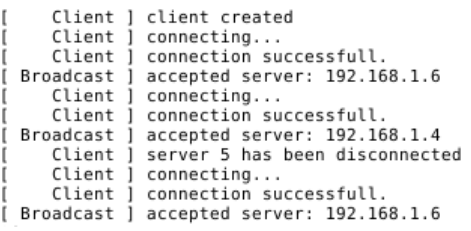
\includegraphics{log_1}
    \caption{Работа участника 1 (процесс-клиент) до прерывания работы}\label{log_1}
\end{figure}
\newpar
На рисунке \ref{log_1} видно, что клиентом обнаружены два участника в сети с IP-адресами
192.168.1.6 и 192.168.1.4, далее следует разрыв соединения с
участником 2 (192.168.1.6) по причине завершения его работы, затем участник 2
снова появляется в сети и снова становится
видимым, далее следует
установление соединения с ним.
\newpar
Допустим, что данный участник 1 по какой-либо причине завершил работу, ниже, на рисунке \ref{log_2} показывается
возобновление его работы. При этом двое других участников снова обнаружены
и, с ними, успешно установлена связь.

\begin{figure}[!hbt]
    \centering
    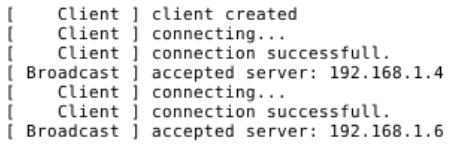
\includegraphics{log_2}
    \caption{Работа участника 1 (процесс-клиент), возобновление работы}\label{log_2}
\end{figure}
\newpar
Сервер в свою очередь производит широковещание, следовательно, его должны
обнаружить остальные участники сети. Ниже, на рисунке \ref{log_3} показано, что два
других участника успешно обнаружили данного участника 1 и установили с
ним соединение. Также на этом же рисунке видно, что с участником 2 потеряна
связь по причине завершения его работы и далее, после возобновления его
работы связь с ним восстанавливается.

\begin{figure}[!hbt]
    \centering
    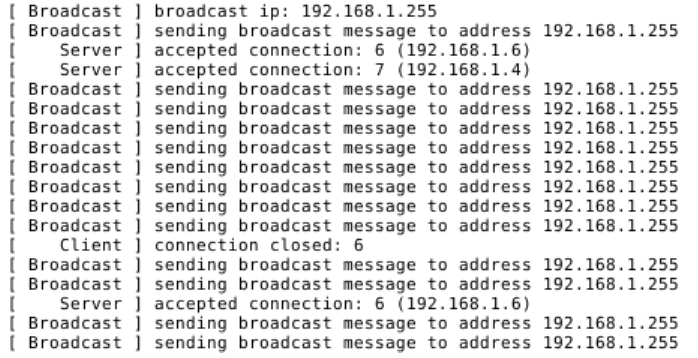
\includegraphics[width=\textwidth]{log_3}
    \caption{Работа участника 1 (процесс-сервер)}\label{log_3}
\end{figure}
\newpar
Рассмотрим работу участника 2 (192.168.1.4). Процесс-клиент участника 2
успешно стартует и успешно устанавливает связь с двумя другими
участниками (рисунок \ref{log_4}). Далее прерывает работу участник 3. После того
как участник 3 возобновил работу соединение устанавливается успешно,
тоже самое можно наблюдать на приведенном выше рисунке \ref{log_1}, с позиции
первого участника.

\begin{figure}[!hbt]
    \centering
    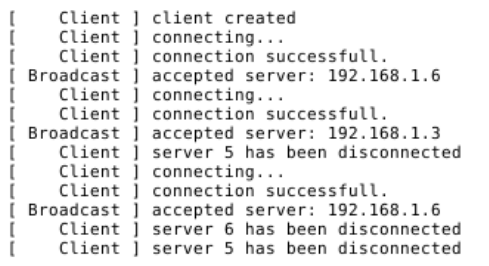
\includegraphics{log_4}
    \caption{Работа участника 2 (процесс-клиент) до прерывания работы}\label{log_4}
\end{figure}
\newpar
Отметим, что данный участник не прерывал своей работы. На рисунке \ref{log_5},
ниже, приведем рисунок с результатами работы процесса-сервера участника 2.

\begin{figure}[!hbt]
    \centering
    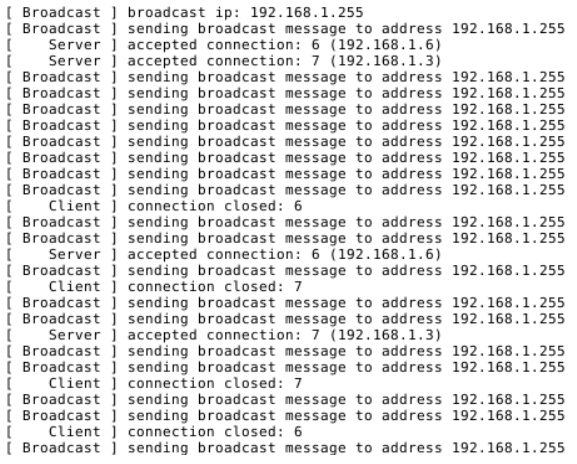
\includegraphics[width=\textwidth]{log_5}
    \caption{Работа участника 2}\label{log_5}
\end{figure}
\newpar
Процесс-сервер успешно запускается и начинает производить
широковещательную рассылку сообщений для того, чтобы другие участники
его обнаружили. Как видно на рисунке \ref{log_5} происходит разрыв связи с двумя
другими участниками, после того как они возобновляют свою работу снова
устанавливается соединение.
\newpar
Рассмотрим работу участника 3. Предположим, что также как и у участника 1
в работе данного участника 3 происходит некоторая ситуация в результате
которой его работа завершается и снова возобновляется. На рисунке \ref{log_6}
приведем пример работы клиента до завершения (прерывания) работы, а на
рисунке \ref{log_7} после возобновления.

\begin{figure}[!hbt]
    \centering
    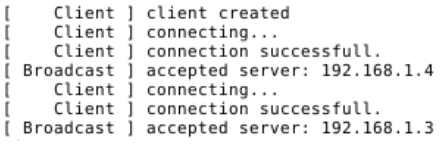
\includegraphics{log_6}
    \caption{Работа участника 3 (процесс-клиент) до прерывания работы}\label{log_6}
\end{figure}
\begin{figure}[!hbt]
    \centering
    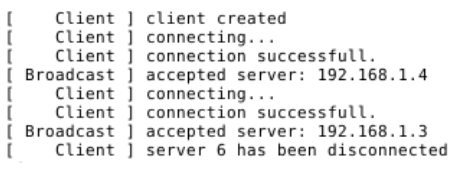
\includegraphics{log_7}
    \caption{Работа участника 3 (процесс-клиент) после возобновления}\label{log_7}
\end{figure}
\newpar
Анализируя приведенные выше результаты работы процесса-клиента
участника 3 видно, что связь устанавливается корректно после запуска и
после возобновления работы участника 3.
\newpar
На рисунке \ref{log_8}, ниже, представлен результат работы процесса-сервера
участника 3.

\begin{figure}[!hbt]
    \centering
    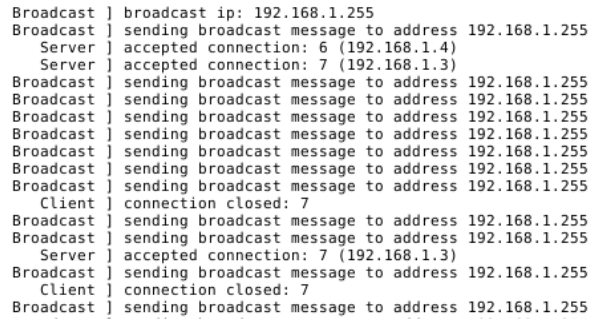
\includegraphics[width=\textwidth]{log_8}
    \caption{Работа участника 3 (процесс-сервер)}\label{log_8}
\end{figure}
\newpar
Как и в предыдущих примерах, видно, что связь устанавливается корректно.
Участники также корректно отображаются в пользовательском приложении,
ниже на рисунках \ref{log_10}, \ref{log_11} и \ref{log_12} приведем примеры панелей «Активность
клиента» для участника 1, участника 2 и участника 3 соответственно.

\begin{figure}[!hbt]
    \centering
    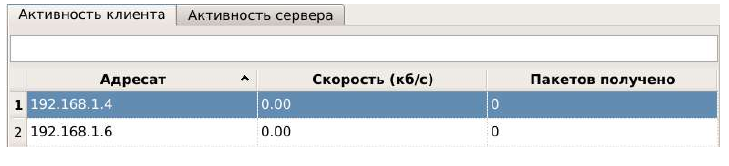
\includegraphics[width=\textwidth]{log_10}
    \caption{Панель <<Активность клиента>> участника 1}\label{log_10}
\end{figure}
\begin{figure}[!hbt]
    \centering
    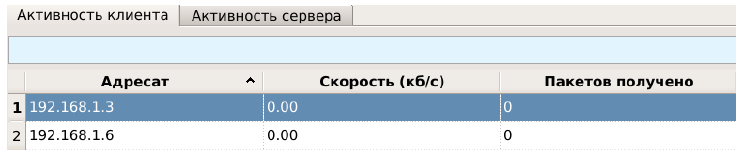
\includegraphics[width=\textwidth]{log_11}
    \caption{Панель <<Активность клиента>> участника 2}\label{log_11}
\end{figure}
\begin{figure}[!hbt]
    \centering
    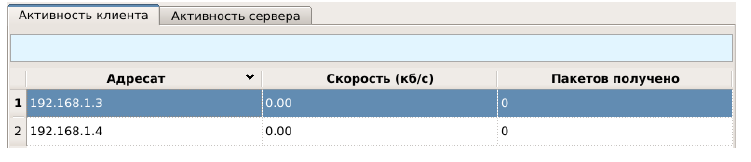
\includegraphics[width=\textwidth]{log_12}
    \caption{Панель <<Активность клиента>> участника 3}\label{log_12}
\end{figure}
\newpar
Было проведено тестирование, из которого можно сделать следующие
выводы:
\begin{enumerate}
    \item обнаружение и установления соединения между участниками
        устанавливается автоматически;
    \item при завершении по каким-либо причинам работы одного из участников,
        работа сети не нарушается, а также это не влияет на работоспособность
        других участников;
    \item при возобновлении работы участников обнаружение и установление
        соединения происходят автоматически;
\end{enumerate}

\subsubsection*{Тестирование запуска демонов}
Процесс-клиент и процесс-сервер являются демонами и должны запускаться
в единственном экземпляре. Попробуем запустить более чем один процесс.
Далее, на рисунке \ref{log_9} показана попытка запуска более чем одного процесса-
клиента и процесса-сервера. Используя команду \texttt{ps –ajx}, которая отображает
демонов, увидим, что были запущены только по одному экземпляру
процессов демонов (рисунок \ref{log_13}). На рисунке \ref{log_14} приведем иллюстрацию
регистрации попытки запуска более чем одного процесса демона.

\begin{figure}[!hbt]
    \centering
    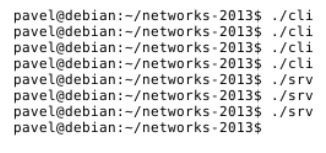
\includegraphics{log_9}
    \caption{Тестирование процесса-демона}\label{log_9}
\end{figure}
\begin{figure}[!hbt]
    \centering
    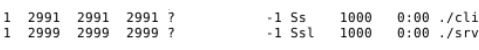
\includegraphics{log_13}
    \caption{Результат команды \texttt{ps -ajx}}\label{log_13}
\end{figure}
\begin{figure}[!hbt]
    \centering
    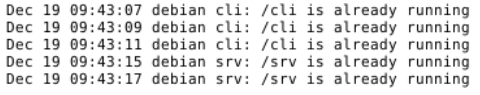
\includegraphics{log_14}
    \caption{Регистрация попытки запуска более чем одного процесса-демона}\label{log_14}
\end{figure}

\subsubsection*{Тестирование передачи файла}
Для тестирования передадим файл \texttt{Favorski\_Kostomarov.djvu} с двух хостов на
третий.
\newpar
Создадим торрент файл, ниже на рисунке \ref{log_15} продемонстрировано создание.
Файл запрашивает участник с IP-адресом 172.20.10.2. У двух других
участников IP адреса 172.20.10.3 и 172.20.10.5, это можно увидеть на том же
рисунке \ref{log_15} во вкладке <<Активность клиента>>. На рисунке \ref{log_16} можно увидеть,
что торрент файл был создан успешно и теперь, данный файл можно
запросить у двух других участников. На рисунке \ref{log_17} можно увидеть, что файл
был передан успешно. Также можно увидеть, сколько пакетов было передано
каждым участником. На рисунках \ref{log_18} и \ref{log_19} можно увидеть вкладку
<<Активность сервера>> двух других участников, при этом отображается имя
переданного файла и число переданных пакетов. На рисунке \ref{log_20} показан
журнал событий, в котором отмечается запуск передачи, на рисунке \ref{log_21} можно
увидеть, что файл был успешно передан, результат заносится в журнал.

\begin{figure}[!hbt]
    \centering
    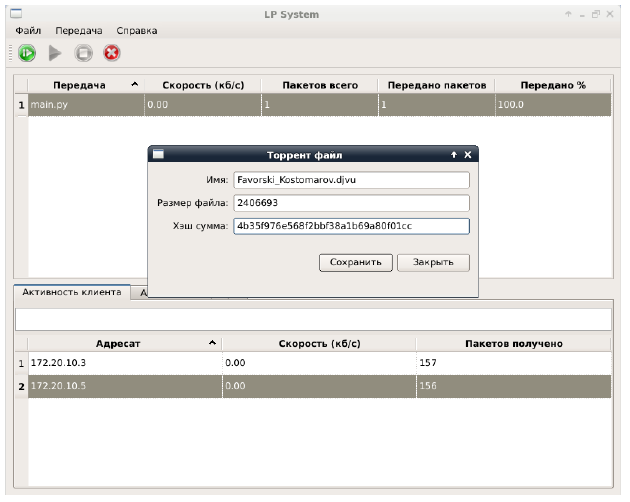
\includegraphics[width=\textwidth]{log_15}
    \caption{Создание торрент-файла}\label{log_15}
\end{figure}
\begin{figure}[!hbt]
    \centering
    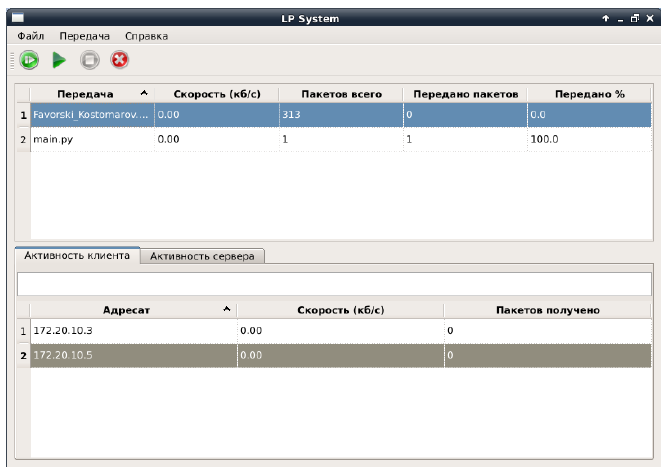
\includegraphics[width=\textwidth]{log_16}
    \caption{Созданный торрент-файл}\label{log_16}
\end{figure}
\begin{figure}[!hbt]
    \centering
    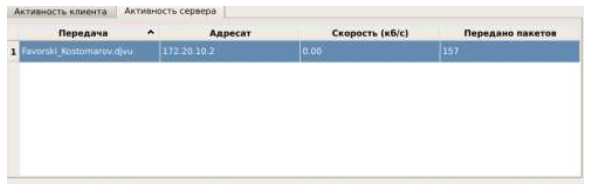
\includegraphics[width=\textwidth]{log_18}
    \caption{Вкладка <<Активность сервера>> участника 1}\label{log_18}
\end{figure}
\begin{figure}[!hbt]
    \centering
    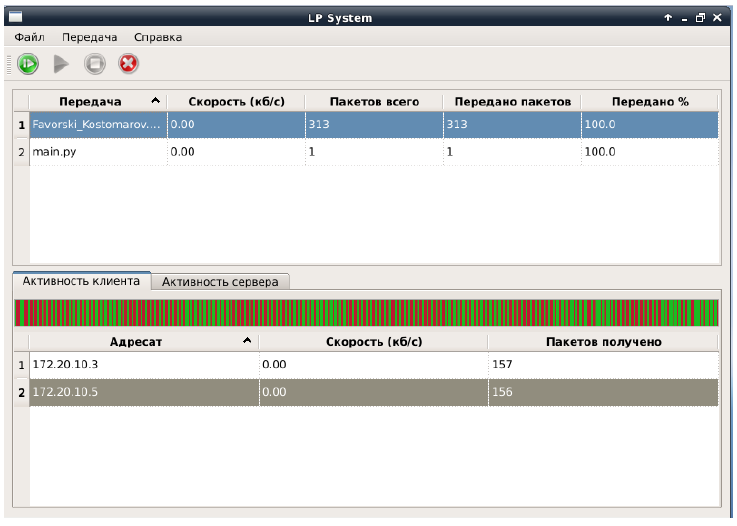
\includegraphics[width=\textwidth]{log_17}
    \caption{Переданный файл}\label{log_17}
\end{figure}
\begin{figure}[!hbt]
    \centering
    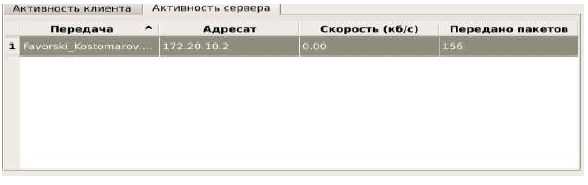
\includegraphics[width=\textwidth]{log_19}
    \caption{Вкладка <<Активность сервера>> участника 2}\label{log_19}
\end{figure}
\begin{figure}[!hbt]
    \centering
    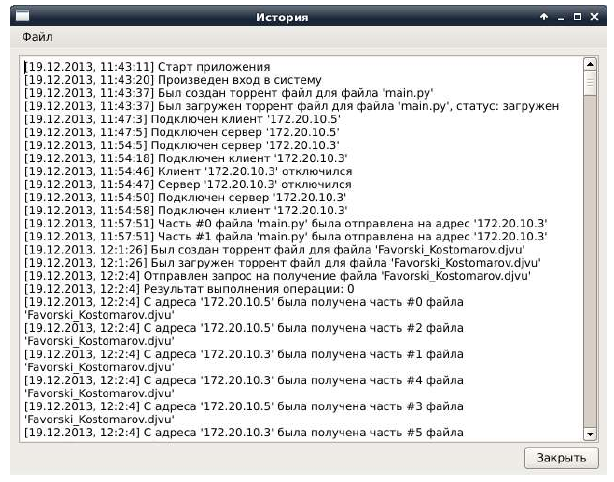
\includegraphics[width=\textwidth]{log_20}
    \caption{Регистрация начала передачи файла}\label{log_20}
\end{figure}
\begin{figure}[!hbt]
    \centering
    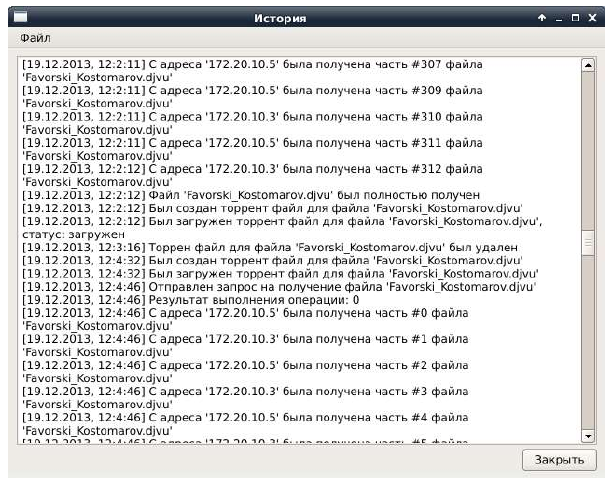
\includegraphics[width=\textwidth]{log_21}
    \caption{Регистрация получения файла}\label{log_21}
\end{figure}

\vfill
\clearpage
\subsection*{Выводы}
\addcontentsline{toc}{subsection}{Выводы}
Был разработан графический интерфейс, который отображает информацию о
передачах и предоставляет пользователю доступ к основным функциям
приложения, а именно:
\begin{enumerate}
    \item создание торрент файлов;
    \item добавление торрент файлов;
    \item запуск, остановка, завершение передач;
\end{enumerate}

Также в приложении имеется журнал, в котором происходит регистрация
основных событий таких как: запуск приложения, возникновение
внештатных ситуаций, добавление нового участника сети, завершение работы
некоторого участника.
\newpar
Приведенные результаты тестирования позволяют сделать вывод о
работоспособности приложения, а также корректную обработку внештатных
ситуаций.


    \setcounter{section}{0}
    \setcounter{subsection}{0}
	\newpage
	\addcontentsline{toc}{section}{\bibname}
	\nocite{*}
    \newsection{Список литературы}
    \printbibliography
	\begin{appendix}
\section*{Приложение А}
\newsection{Приложение А}
\addcontentsline{toc}{section}{Приложение А}
В приложении приводятся основные прототипы пользовательских функций,
структур и некоторых типов данных.
\subsubsection*{Прототипы функций и структуры, используемые сервером}
Структура приведенная ниже описывает характеристики куска файла, такие
позиции начала и конца куска, содержит сам кусок, имя файла и указатель
на объект \texttt{FILE}. Используемые константы:
\begin{itemize}
    \item \texttt{CACHED\_PIECES\_COUNT}~-- число кусков находящихся в кэше.
    \item \texttt{DATA\_BLOCK\_LEN}~-- размер куска файла.
\end{itemize}
\begin{lstlisting}
struct file_cache {
    unsigned char data[CACHED_PIECES_COUNT * DATA_BLOCK_LEN];
    piece_id_t start_piece;
    piece_id_t end_piece;
    char name[DATA_BLOCK_LEN];
    FILE *file;
};
\end{lstlisting}

Структура, которая реализует очередь кусков файлов.
\texttt{MAX\_TRANSMISSIONS}~-- максимальное число передач.
\begin{lstlisting}
struct files_queue {
    char positions[MAX_TRANSMISSIONS];
    struct file_cache cache[MAX_TRANSMISSIONS];
    int count;
};
\end{lstlisting}

Функция, которая обрабатывает сообщение переданное клиентом.\\
\texttt{int process\_client\_message(int sender\_sock, const char *msg, size\_t count);}

Функция ниже используется для обмена сообщениями с пользовательским
приложением.\\
\texttt{void setup\_gui\_acts(struct gui\_actions *acts);}

\subsubsection*{Прототипы функций и структуры, используемые клиентом}
Структура описывает кусок, который выбивается из структуры ниже
\begin{lstlisting}
struct file_udata_t {
    piece_id_t piece_id;    \\ Индекс куска файла
    piece_len_t piece_len;  \\ Текущий размер куска
    unsigned char data[DATA_BLOCK_LEN]; \\ Кусок данных
};
\end{lstlisting}

Структура описывает блок данных для сброса на жесткий диск.
\begin{lstlisting}
struct file_data_t {
    piece_id_t s_piece;
    piece_id_t f_piece;
    int pieces_copied;
    size_t full_size;
    unsigned char data[CACHED_PIECES_COUNT* DATA_BLOCK_LEN];
};
\end{lstlisting}

Структура объединяет структуры выше, чтобы не передавать лишние па-
раметры
\begin{lstlisting}
struct file_full_data_t {
    struct file_data_t data;
    struct file_udata_t udata[CACHED_QUEUE_LEN];
};
\end{lstlisting}

Структура описывает одно активное соединение (подключение)
\begin{lstlisting}
struct active_connection {
    int srv_sock;
    int timeout;
    int transmission_id;
    int status;
    piece_id_t piece_id;
    file_id_t file_id;
    pack_id_t pack_id;
    struct file_full_data_t *data;
    struct active_connection *next;
    struct active_connection *prev;
};
\end{lstlisting}

Список всех активных соединений (подключений)
\begin{lstlisting}
struct active_connections {
    struct active_connection *q_head;
    struct active_connection *q_tail;
};
\end{lstlisting}

Структура для описания части файла, которую необходимо запросить
\begin{lstlisting}
struct pieces_queue {
    piece_id_t max_piece_num; \\ Максимальный номер куска
    piece_id_t cur_piece; \\ Содержит минимальный не запрошенный номер куска
    signed int max_failed_piece_num; \\ Максимальный номер куска в failed_pieces
    piece_id_t failed_pieces[MAX_PIECES_COUNT]; \\ Содержит неполученные куски файла
    piece_id_t flushed_pieces_count; \\ Число записанных на диск кусков
};
\end{lstlisting}

Структура определяет одну активную передачу
\begin{lstlisting}
struct transmission {
    FILE *file;
    char filename[FILE_NAME_MAX_LEN];
    unsigned char filesum[MD5_DIGEST_LENGTH];
    unsigned short status;
    size_t filesize;
    struct pieces_queue pieces;
};
\end{lstlisting}

Структура описывает список всех активных передач
\begin{lstlisting}
struct transmissions {
      struct transmission trm[MAX_TRANSMISSIONS];
      unsigned char openned_trms[MAX_TRANSMISSIONS];
      unsigned int count; \\ Число закрытых передач
};
\end{lstlisting}

Функция обрабатывает сообщения, полученные от сервера\\
\texttt{int process\_srv\_message(int sock, const char *msg, size\_t len);}
\newpar
Функция, реализующая работу диспетчера\\
\texttt{void main\_dispatcher();}
\newpar
Функция, запускающая посылку файла\\
\texttt{int receive\_file(const char *filename, const
unsigned char *hsum, unsigned long fsize, const struct sockets\_queue *q);}
Функция для обмена сообщениями с пользовательским интерфейсом\\
\texttt{void setup\_gui\_acts(struct gui\_actions *acts);}
\subsubsection*{Прототипы функций модуля Network}
Функция, которая запускает процесс-сервер\\
\texttt{int start\_server(socket\_callback process\_cli\_msg\_callback);}
\newpar
Функция, которая запускающая процесс-клиент\\
\texttt{int start\_client(socket\_callback
process\_srv\_msg\_callback,
queue\_dispatcher dispatcher, struct sockets\_queue *q);}
\newpar
Функция, используемая для пересылки данных\\
\texttt{int send\_data(int sock, char *buf, int len, int flags);}
\newpar
Функция, необходимая для обмена сообщениями
с пользовательским приложением\\
\texttt{void setup\_gui\_msgs(struct gui\_actions *acts);}
\subsubsection*{Прототипы функция для обработки сообщений}
Десериализация, полученного сообщения от клиента\\
\texttt{int encode\_cli\_msg(struct cli\_fields *fields, const char *msg, int
msg\_len);}
\newpar
Сериализация сообщения посылаемого клиенту\\
\texttt{int decode\_cli\_msg(const struct cli\_fields *fields, char *msg);}
\newpar
Десериализация, полученного сообщения от сервера\\
\texttt{int encode\_srv\_msg(struct srv\_fields *fields, const char *msg, int
msg\_len);}
\newpar
Сериализация сообщения посылаемого серверу\\
\texttt{int decode\_srv\_msg(const struct srv\_fields *fields, char *msg);}
\newpar
Декодирование ошибок (интерпретация)\\
\texttt{void decode\_proto\_error(perror\_t e, char *s, int max\_len);}

\subsubsection*{Callback-функции для обмена сообщениями с пользовательским приложением}
\begin{lstlisting}
struct gui_actions {
    gui_recv_callback start_trm;
    gui_recv_callback stop_trm;
    gui_recv_callback terminate;
    gui_send_callback answer;
    gui_send_callback package_sent;
    gui_send_callback package_received;
    gui_send_callback server_added;
    gui_send_callback client_added;
    gui_send_callback server_removed;
    gui_send_callback client_removed;
    gui_send_callback file_received;
    int sock;
};
\end{lstlisting}

Опишем смысл функций в порядке следования в структуре:

\begin{enumerate}
    \item начать передачу
    \item остановить передачу
    \item завершить работу
    \item ответить
    \item отправленные пакеты
    \item полученные пакеты
    \item добавление клиента
    \item добавление сервера
    \item удаление клиента
    \item удаление сервера
    \item файл получен
\end{enumerate}

Следующая структура хранит массив активных сокетов
\begin{lstlisting}
struct sockets_queue {
    int sockets[MAX_CONNECTIONS];
    in_addr_t addrs[MAX_CONNECTIONS];
    int count;
};
\end{lstlisting}

Выше были приведены основные прототипы и структуры данных, которые не
были указаны в технологическом разделе.

\section*{Приложение Б}
\newsection{Приложение Б}
\addcontentsline{toc}{section}{Приложение Б}
В данном приложении будут представлены исходные коды некоторых программных модулей проекта.
\subsection*{Исходные коды модуля \texttt{proto.c}}
\addcontentsline{toc}{subsection}{Исходные коды модуля \texttt{proto.c}}
\lstinputlisting[language=C]{../backend/proto.c}
\subsection*{Исходные коды модуля \texttt{srv.c}}
\addcontentsline{toc}{subsection}{Исходные коды модуля \texttt{srv.c}}
\newsection{Приложение Б}
\lstinputlisting[language=C]{../backend/srv.c}
\end{appendix}

\end{document}
